Estimating dense 3D geometry from 2D images is an important problem with
applications to robotics, autonomous driving, and medical imaging. Depth maps
are a common representation of scene geometry and are useful precursors to
higher-level scene understanding tasks such as pose estimation and object
detection. Additionally, many computer vision tasks rely on depth sensing,
including navigation~\cite{geiger2013vision}, semantic
segmentation~\cite{gupta2013perceptual,ren2012rgb,silberman2012indoor}, 3D
object
detection~\cite{gupta2014learning,lin2013holistic,shrivastava2013building,song2014sliding,song2016deep},
and 3D object
classification~\cite{maturana2015voxnet,qi2016volumetric,wu20153d}.

\begin{figure}[t]
  \centering
  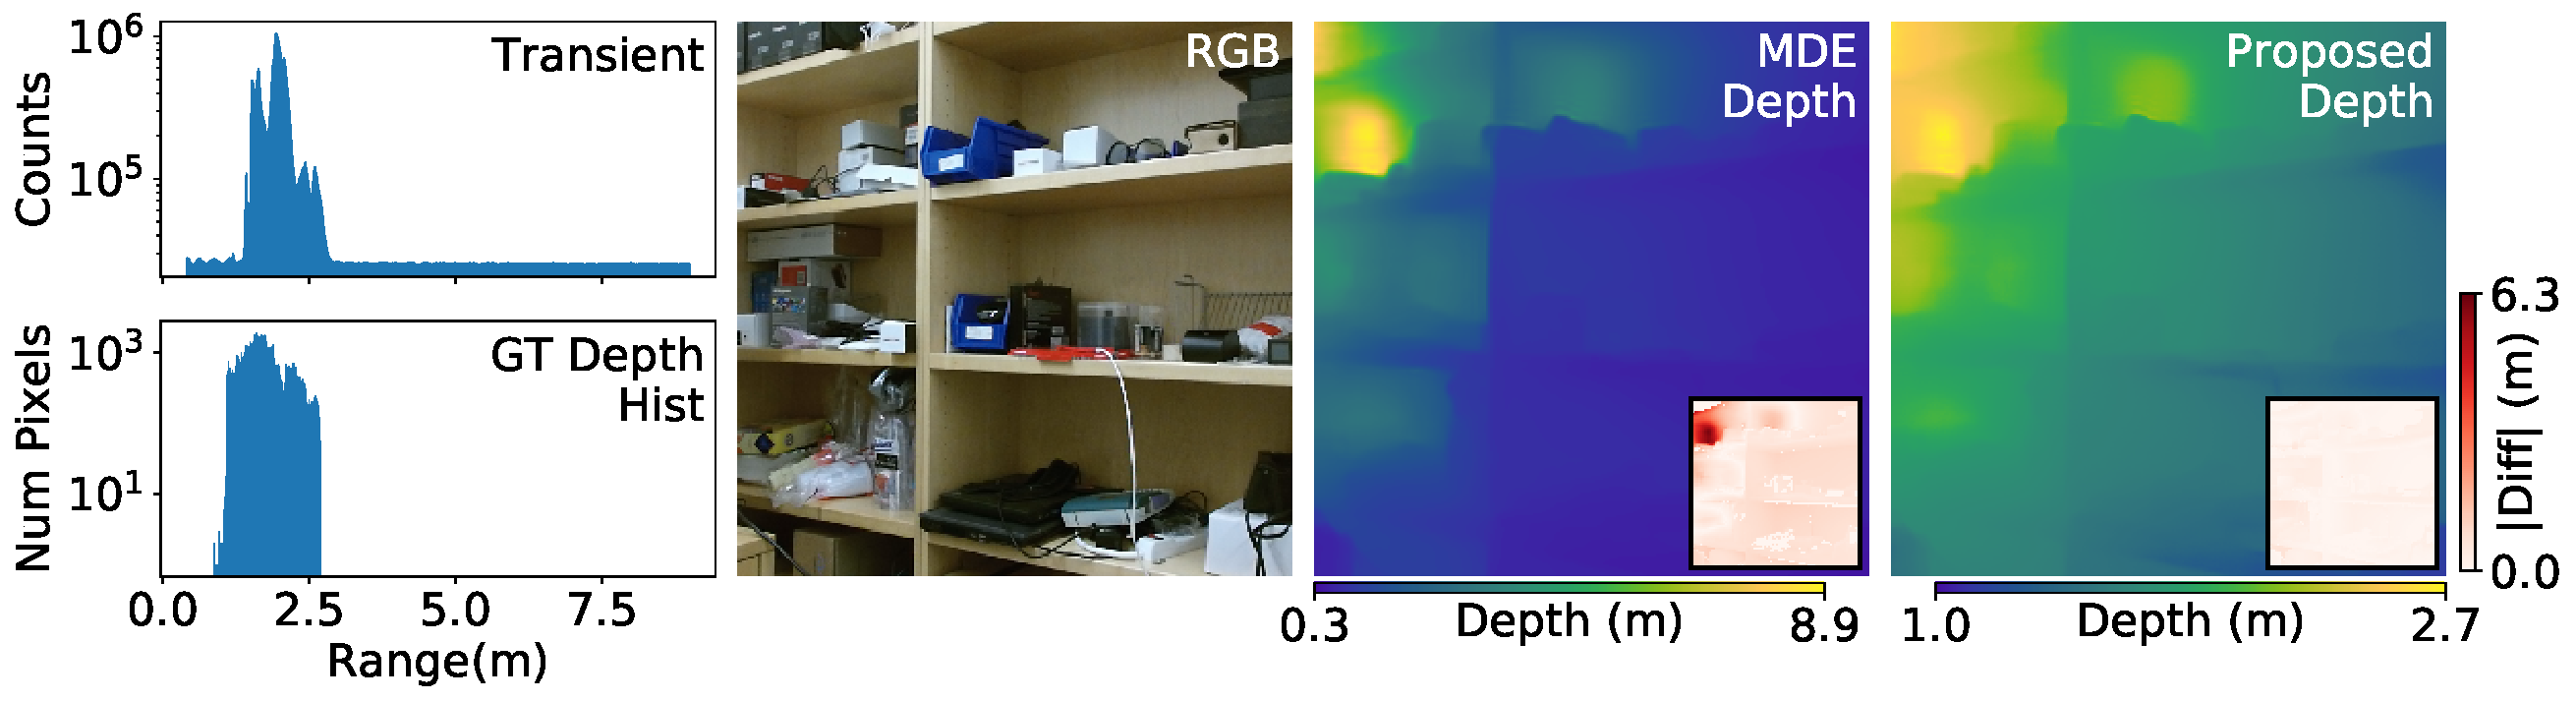
\includegraphics[width=\columnwidth]{teaser_eccv.pdf}
  \caption{Monocular depth estimation predicts a depth map (second from right) from a
    single RGB image (second from left). The ill-posedness of the problem prevents
    reliable absolute depth estimation, resulting in large errors (inset images).
    The proposed method uses a \edit{single transient measurement aggregating
      the time-of-flight information of the entire scene (leftmost)} to correct
    the output of the depth estimation and optimize the quality of the
    estimated absolute depth (rightmost).}
  \label{fig:teaser}
\end{figure}

Traditional depth sensing techniques include those based on stereo or multiview,
active illumination, camera motion, or focus cues~\cite{szeliski2010computer}.
However, each of these techniques has aspects that may make their deployment
challenging \edit{in certain scenarios}. For example, stereo or multiview techniques require multiple
cameras, active illumination techniques may have limited resolution or require
time-consuming scanning procedures, and other techniques require camera motion
or multiple exposures at different focus distances.


One of the most promising approaches to overcoming these challenges is monocular
depth estimation (MDE), which requires only a single RGB image from a
conventional camera to recover a dense depth
map~\cite{Alhashim2018,Eigen2014,Fu2018,Laina2016,Saxena2006}. Recent approaches
to MDE employ neural networks that learn to predict depth by exploiting
\edit{pictorial depth} cues such as perspective, occlusion, shading, and relative
object size. While such models have significantly improved over recent years,
MDE approaches to date are incapable of reliably estimating absolute distances
in a scene due to the inherent scale ambiguities of monocular image cues.
Instead, these models excel in predicting ordinal depth, or the relative
ordering of objects in a scene~\cite{Eigen2014,Fu2018}. Interestingly, Alhashim
and Wonka~\cite{Alhashim2018} recently showed that if the median ground truth
depth of the scene is known, the initial output of a MDE network can be
corrected to produce accurate absolute depth.


%For example, a larger object at a far distance to the camera results in the
%same 2D camera image as a smaller object of the same type that is closer to the
%camera. Therefore, MDE approaches to date are incapable of reliably estimating
%absolute distances of a scene. Interestingly, Alhashim and
%Wonka~\cite{Alhashim2018} recently showed that if the MDE network has oracle
%access to the ground truth median depth, then correcting the output of the CNN
%to match this median depth produces accurate absolute depth maps both
%qualitatively and quantitatively.


% move to discussion
%However, traditional approaches to depth estimation, such as stereo, suffer
%from lower performance when confronted with small angles or faraway objects.
%More exotic approaches use FMCW or time-of-flight LiDAR technologies, but these
%approaches are currently expensive and bulky.


%The most promising solution to these issues uses deep learning and
%convolutional neural networks to perform \textit{monocular depth estimation},
%estimating dense depth maps from single RGB images.  However, this problem is
%underconstrained due to \textit{inherent scale ambiguity}, the unresolvable
%tradeoff between size and distance in single images. In practice, this issue
%commonly manifests itself in many monocular depth networks, and indeed, Wonka
%et. al. (cite) showed that if the method has oracle access to the ground truth
%median depth, then correcting the output of the CNN to match this median depth
%produces better depth maps both qualitatively and quantitatively.




Although access to the median ground truth depth is impossible in a realistic
scenario, low-cost sensors capable of capturing aggregated depth information
from a scene are readily available. For example, the proximity sensor on recent
generation Apple iPhones uses a low-power pulsed light source and a
single-pixel \edit{time-resolved detector} %, single-photon avalanche diode (SPAD) 
to sense distance to an
object directly in front of the phone. %SPADs 
\edit{
Time-resolved detectors, such as avalanche photon diodes (APDs) or single-photon
avalanche diodes (SPADs), can measure the full waveform of time-resolved incident
radiance at each pixel (Fig.~\ref{fig:teaser}). These detectors form the
backbone of modern LiDAR
systems~\cite{Kirmani:2014,Li:2019,pawlikowska2017single}. However,
single-photon sensor arrays} have
not yet been used for 3D imaging on consumer electronics, primarily because the requirement for
ultra-fast timing electronics makes it difficult to produce high-resolution
arrays at low cost and because the scanning requirement for single-pixel
systems introduces a point of mechanical failure and complicates
high-resolution, high-framerate imaging.


%Individual SPADs are easy to fabricate and sufficiently cost-effective to be
%deployed in consumer electronics. When coupled with high-power pulsed lasers,
%they also form the backbone of emerging single-photon LiDAR
%systems~\cite{Kirmani:2014,pawlikowska2017single,Li:2019}. However, the
%required ultra-fast time-stamping electronics make it difficult to fabricate
%high-resolution SPAD arrays at low cost. Moreover, the scanning requirement for
%single-pixel systems precludes high-resolution, high-framerate depth mapping
%and is a barrier to integration in small consumer electronics.


Here, we propose to use a single-pixel \edit{time-resolved detector} and pulsed light source in an
unconventional way: rather than optically focusing them to record the distance
to a single scene point, we diffuse the emitted light and \edit{aggregate the reflected light over the
entire scene with the detector}. The resulting \edit{transient} measurement
resembles a histogram of the scene depth and we demonstrate that this can be
used to achieve accurate absolute depth when combined with the estimate of
\edit{any monocular depth estimator in a post-processing step}
(Fig.~\ref{fig:teaser}).


%Technically, a diffused SPAD does not record a true depth histogram, but a
%transient that is affected by square-distance falloff of the backscattered
%light, spatially varying reflectance of the scene, ambient photons, and
%detector noise. Nevertheless, we can interpret the measurements of a
%single-pixel SPAD as something similar to a depth histogram.


%In this paper, we go further and show that by augmenting the RGB image with a
%histogram of global image depths, we can achieve substantially improved
%performance (and generalizability) over state-of-the-art monocular depth
%estimators. By performing an exact, weighted histogram matching on the output
%depth map of the depth estimator, we can match the depth histogram of the scene
%to the depth histogram of our estimate. This histogram matching is described in
%(cite) and is flexible enough to accommodate different pixel reflectances in
%the RGB image. Finally, this histogram can be captured relatively inexpensively
%using only a single pixel single-photon avalanche diode (SPAD) and pulsed laser
%illumination diffused over the field of view, representing a significant
%improvement in cost and simplicity over multi-pixel LiDAR arrays with expensive
%scanning mechanisms. It is worth noting that SPADs of this type have already
%made their way into existing smartphones, such as the iPhone X, and will likely
%play a role in future mobile sensing platforms as well.



% move to discussion


To this end, we develop a sensor fusion strategy that processes the ordinal
depth computed by a monocular depth estimator to be consistent with the
measurements captured by the \edit{aggregated time-resolved} detector. We demonstrate in extensive
simulations that our approach achieves substantial improvements in the quality
of the estimated depth maps, regardless of which specific depth estimator is
used. \edit{Moreover, we build a camera prototype that combines an RGB camera and a single-pixel time-resolved detector and use it to validate the proposed depth estimation technique.} % With this work, we present a practical way to disambiguate depth estimation with RGB images using minimal additional sensing hardware.

In summary, we make the
following contributions:
%
\begin{itemize}
	\item We propose augmenting an RGB camera with a global depth histogram aggregated by a time-resolved detector to address scale ambiguity in MDE.	
  \item We analyze this approach on indoor scenes using the NYU Depth v2 dataset and demonstrate that our approach is able to resolve scale ambiguity while being fast and easy to implement.
	\item We build a prototype camera and evaluate its efficacy on captured data, assessing both the quality and the ability of our method to help generalization of monocular depth estimators across scene types. 
\end{itemize}


%\edit{\emph{Overview of Limitations:} our prototype camera uses a scanned SPAD and digitally aggregates the captured transients to emulate a single optically diffused measurement. The benefit of this approach is access to ground truth depth, allowing us to evaluate the efficacy of our method with measured data. However, when operating SPADs in certain conditions, they may observe a nonlinear aggregation effect known as pileup. In these conditions, the aggregated measurements may differ from a single optically diffused measurement. Yet, we experimentally verify that digitally and optically aggregated measurements captured with our system are very similar and pileup could also be computationally corrected~\cite{Heide:2018,Rapp:2019}, although we did not attempt this.} 

%\edit{Our method is not without limitations. It still requires a laser and single-pixel LiDAR detector and is sensitive to ambient photons, which limit the maximum range. Being a variant of histogram matching, our method is not able to resolve ordinal depth errors (errors where an object is wrongly placed closer or farther relative to another object). In spite of these limitations, we find that our method performs remarkably well in practice.}

